\documentclass{article}
\usepackage{graphicx}
\usepackage{circuitikz}
\usepackage{float}

\title{T-Junction Traffic Controller Design}
\author{Arnav Yadnopavit EE24BTECH11007\\Prajwal EE24BTECH11051\\Shivam Shilvant EE24BTECH11057}
\date{\today}

\begin{document}

\maketitle

\section{Introduction}
Design of an intelligent traffic control system for T-junctions with:
\begin{itemize}
    \item Independent traffic light control for two directions (T1 and T2)
    \item Pedestrian walk signals with warning buzzer
    \item Emergency vehicle priority
    \item Turn signal management
\end{itemize}

\section{Design Architecture}

\subsection{State Machines}
\begin{figure}[h]
\centering
\begin{tikzpicture}[->,>=stealth',shorten >=1pt,auto,node distance=2.5cm]
    \node[state] (R) {Red};
    \node[state] (G) [right of=R] {Green};
    \node[state] (GT) [right of=G] {Green+Turn};
    \node[state] (O) [below of=GT] {Orange};
    \node[state] (Y) [left of=O] {Yellow};
    
    \path (R) edge node {Timer=0} (G)
          (G) edge node {Timer=0} (GT)
          (GT) edge node {Timer=0} (O)
          (O) edge node {Timer=0} (Y)
          (Y) edge node {Timer=0} (R);
\end{tikzpicture}
\caption{State machine diagram for each traffic direction}
\end{figure}

\subsection{Key Features}

\subsubsection{Turn Signal Management}
\begin{itemize}
    \item Added special state (GREEN\_WITH\_TURN)
    \item T1 gets right turn signal, T2 gets left turn signal
    \item Turn phase occurs after main green phase
    \item Ensures no green light conflicts between T1 and T2
\end{itemize}

\subsubsection{Emergency Handling}
\begin{itemize}
    \item Asynchronous detection (immediate response)
    \item 10-time unit hold period
    \item Left emergency stops T1 only
    \item Right emergency stops both T1 and T2
\end{itemize}

\subsubsection{Safety Interlocks}
\begin{itemize}
    \item T2 checks T1 state before turning green
    \item Minimum yellow/orange times for safe transitions
    \item Physical impossibility for conflicting green lights
\end{itemize}

\section{Timing Diagram}
\begin{figure}[H]
\centering
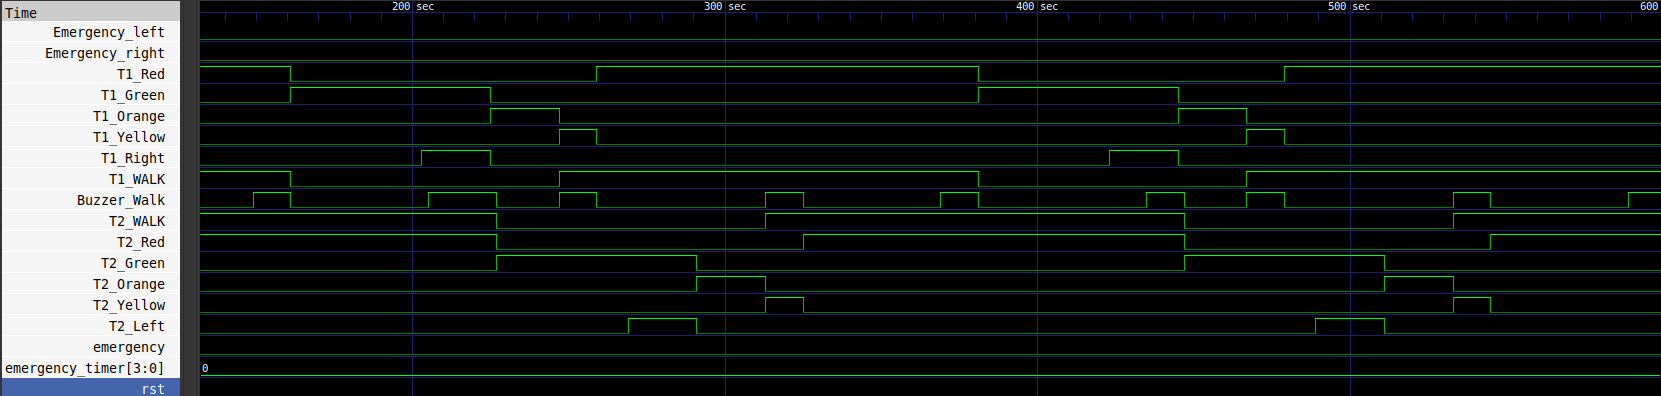
\includegraphics[width=\textwidth]{figs/test.png}
\caption{Example timing sequence showing normal signal phases}
\end{figure}


\section{Implementation Details}

\subsection{Parameters}
\begin{tabular}{|l|l|}
\hline
Parameter & Value (time units) \\
\hline
Red Time & 60 \\
Green Time & 20 \\
Turn Time & 10 \\
Yellow Time & 5 \\
Orange Time & 10 \\
Emergency Time & 10 \\
Buzzer Time & 5 \\
\hline
\end{tabular}

\subsection{Verilog Module Breakdown}
\begin{itemize}
    \item Two independent but synchronized state machines
    \item Asynchronous emergency override
    \item Combinational output logic
    \item Configurable timing parameters
\end{itemize}

\section{Conclusion}
The design meets all requirements while ensuring:
\begin{itemize}
    \item Safe operation through state machine interlocks
    \item Responsive emergency handling
    \item Clear turn signal indication
    \item Predictable timing behavior
\end{itemize}

\end{document}
